% star_reacher scientific report (FR-30) --- AIAA-style structure on the stock
% article class. Build: latexmk -pdf -halt-on-error -interaction=nonstopmode
% (wrapped by `star docs`). Every figure is regenerated by a committed script
% from committed/seeded run logs (scripts/figures/casestudy_figures.py), so the
% paper is itself a regression artifact; sections whose external validation is
% deferred say so plainly rather than inventing results.
\documentclass[10pt]{article}

\usepackage[T1]{fontenc}
\usepackage[utf8]{inputenc}
% Times text and math (mathptmx, texlive-fonts-recommended) approximates the
% AIAA journal look with stock packages only.
\usepackage{mathptmx}
\usepackage[margin=1in]{geometry}
\usepackage{amsmath}
\usepackage{booktabs}
\usepackage{siunitx}
\usepackage{graphicx}
% The astronomical unit under a private macro name (not \au, which some
% packages define) so the case-study text can quote heliocentric distances in
% au without a naming clash; siunitx does not predefine it as an SI unit.
\DeclareSIUnit\astrounit{au}
\usepackage[hidelinks]{hyperref}
% biblatex is loaded after hyperref per the biblatex package documentation.
\usepackage[backend=biber,style=numeric,sorting=nyt]{biblatex}
\addbibresource{references.bib}

% \starversion is overwritten at build time by version.tex, regenerated by
% .latexmkrc from `git describe --always`, mirroring the math library's
% version mechanism so both artifacts trace to the same revision.
\providecommand{\starversion}{unknown}
\InputIfFileExists{version.tex}{}{}

\title{\texttt{star\_reacher}: A Small, Deterministic Six-Degree-of-Freedom
  Space-Mission Simulator with Derived, Cited, and Validated Physical Models}
\author{Melvin Hoyer III}
% Version string instead of a calendar date keeps rebuilds of one revision
% textually identical (SOURCE_DATE_EPOCH reproducibility goal).
\date{Version \texttt{\starversion}}

\begin{document}

\maketitle

\begin{abstract}
\texttt{star\_reacher} is a deterministic six-degree-of-freedom space-mission
simulator for launch vehicles, satellites, and lunar and Mars missions, built
as a small C++17/Eigen compute core behind a Python analysis frontend. Its
design principle is scientific fidelity at minimal size: every physical model
carries a first-principles derivation, explicit domain-of-validity bounds, and
machine-checked validation evidence in a companion mathematical model library,
and the same inputs on the same binary always produce bit-identical outputs,
gated in continuous integration by cryptographic hash with no tolerance. The
simulator targets hardware from a Raspberry Pi~5 to a desktop workstation and
carries artificial-intelligence and machine-learning navigation hooks --- a
major-cycle stepping API, seeded sensor emulation, and a
guidance-navigation-control plugin interface --- designed in from the first
commit. This report describes the architecture, the physical-model set, the
seven-layer verification and validation approach and its measured results, and
two representative case studies (a translunar transfer and an Earth--Mars
transfer) whose figures are regenerated bit-for-bit from committed seeds. The
acceptance suite passes \num{29} of \num{29} checks; seven frozen cross-tool
comparisons are measured, every one inside its gate; and the work that remains
--- a long-arc cross-platform divergence re-measurement and the
Raspberry~Pi~5 hardware qualification --- is identified honestly as pending.
\end{abstract}

\section{Introduction and Related Tools}
\label{sec:intro}

High-fidelity astrodynamics and flight-simulation tools broadly divide into
heavyweight mission-analysis suites, whose models are difficult to audit end to
end, and approachable simulators that trade physical rigor for accessibility.
\texttt{star\_reacher} targets the gap between them: a small, fully auditable,
bit-reproducible truth-model simulator in which every logged quantity traces to
a derived and cited model with recorded validation evidence. The project
validates against established tools rather than competing with them: NASA's
General Mission Analysis Tool (GMAT)~\cite{hughes2014} is the primary
cross-tool baseline, with Orekit~\cite{maisonobe2010} as the tie-breaker and as
the primary baseline for models GMAT does not implement. The classical
astrodynamics on which the physical models rest follows standard references,
principally Vallado~\cite{vallado2013}, Battin~\cite{battin1999}, and
Montenbruck and Gill~\cite{montenbruck2000}; the attitude formulation follows
Markley and Crassidis~\cite{markley2014}; and the navigation substrate follows
Groves~\cite{groves2013} and Titterton and Weston~\cite{titterton2004}.

The design goals are four. First, a truth-model six-degree-of-freedom (6DOF)
capability: full rigid-body translational and rotational dynamics with
time-varying mass properties, suitable as ground truth for guidance,
navigation, and control (GNC) and for navigation research. Second, scrutinized
scientific fidelity: every model carries a first-principles derivation, an
explicit domain of validity, and validation evidence. Third, determinism as a
feature: bit-identical reruns on the same platform and binary, with bounded and
published cross-platform divergence. Fourth, minimality without fidelity loss:
the linear-algebra library Eigen is the only mandatory core dependency, and the
installed runtime dependency set and per-platform wheel size are both enforced
in continuous integration.

\section{Architecture}
\label{sec:architecture}

The system is split by a single boundary rule: everything inside the
deterministic time loop is C++, and everything before the initial epoch or
after the final epoch is Python. The C++17 core --- whose only mandatory
dependency is Eigen --- owns the equations of motion, the force and torque
models, the integrators, event detection, the sensor models, the
pseudorandom-number streams, and the binary log writer; it never parses text,
touches the network, or reads the clock. The Python package owns configuration
validation and canonicalization, Monte Carlo orchestration, the log loader and
exporters, plotting, playback, and the documentation build. The two halves meet
at a pybind11 binding that passes a typed, hashed configuration in and a
self-describing versioned binary log (SRLOG) out.

The log header embeds the resolved-configuration SHA-256, the binary's git
hash, and the master random seed, binding every output to its exact inputs. The
channel dictionary makes the file self-describing; minor format versions add
channels that older readers ignore, while major versions break loudly.
Reserved navigation and sensor channel groups, present from the first commit,
let the later AI/ML phases populate estimator and sensor channels without a
format break.

Determinism is a contract, not an aspiration. The core loop is single-threaded
with a fixed force-summation order; floating-point contraction and fast-math
optimizations are disabled at the compiler level; the pseudorandom streams are
core-owned and seeded per subsystem; and no host or wall-clock data enters the
log body. Same-platform bit-identity is enforced in continuous integration by
comparing SHA-256 hashes of repeated runs with no tolerance, and cross-platform
divergence is bounded and measured rather than assumed away.

\section{Physical Models}
\label{sec:models}

Every physical model is documented in the companion mathematical model library,
where each chapter follows a fixed six-section template: purpose; assumptions
and domain of validity, with out-of-domain behavior stated and matched to the
code; a complete derivation with every non-original result cited; discretization
and implementation notes with equation-label-to-code traceability; a
validation-evidence table of machine-checked test identifiers; and references.
A manifest lint enforces accretion: a core model module without its chapter
fails the build. The model set is complete through the current phase; Table~%
\ref{tab:models} summarizes it and names the library chapter that derives each
group. Cross-references are given by chapter title rather than by number because
the model library is a separate document; the two artifacts are built together
by \texttt{star docs} and carry the same version string.

\begin{table}[htbp]
\centering
\caption{Physical-model set and the mathematical-model-library chapter deriving
  each group. Both documents are built by \texttt{star docs} and share one
  version string.}
\label{tab:models}
\small
\begin{tabular}{@{}p{0.34\linewidth}p{0.58\linewidth}@{}}
\toprule
Model group & Companion-library chapter(s) \\
\midrule
Time systems (TAI/UTC/TT/TDB) & Time Systems \\
Reference frames (GCRF, IAU 2006/2000B Earth-fixed, Moon PA, Mars IAU),
  per the IERS Conventions~\cite{iers2010} &
  Reference Frames; Rotations and Attitude \\
Ephemerides (trimmed DE440 Chebyshev subset~\cite{park2021}) & Ephemerides \\
Integrators (RK4, RKF7(8)~\cite{fehlberg1968,hairer1993}, dense output) &
  Numerical Integration \\
Event detection (Brent root-finding on dense output) & Event Detection \\
Harmonic gravity (Pines normalized, Earth/Moon/Mars fields) & Gravity \\
Third-body perturbation (Battin cancellation-safe form~\cite{battin1999}) &
  Third-Body Perturbation \\
Solar radiation pressure (cannonball, conical shadow) &
  Solar Radiation Pressure \\
Atmospheres (USSA76~\cite{ussa1976}, Harris--Priester, Mars table) and drag &
  U.S. Standard Atmosphere 1976; Harris--Priester; Mars Atmosphere; Drag \\
Vehicle mass properties, propulsion, actuators, aerodynamics &
  Mass Properties; Propulsion; Actuators; Aerodynamics \\
Rigid-body 6DOF attitude with gravity-gradient torque~\cite{markley2014} &
  Rigid-Body Dynamics; Gravity-Gradient Torque; Vehicle 6DOF \\
Sensors (IMU, optical, radio, camera hook)~\cite{titterton2004,groves2013} &
  IMU Sensors; Optical Sensors; Radio Sensors; Camera Hook \\
GNC components and error-state EKF~\cite{groves2013} &
  Built-in GNC Components; Extended Kalman Filter \\
\bottomrule
\end{tabular}
\end{table}

The Earth orientation deliberately neglects polar motion and sets the
UT1$-$UTC offset to zero (a user-suppliable constant), a documented
domain-of-validity bound rather than an omission; the same convention is
applied to both sides of the cross-tool comparisons in Section~\ref{sec:vv}. On-%
orbit aerodynamic, solar-radiation-pressure, and magnetic disturbance torques
are explicit non-goals with magnitude bounds recorded in the model library;
gravity-gradient torque is modeled.

\section{Verification and Validation Approach}
\label{sec:vv}

Verification and validation proceed in seven machine-checkable layers, each
carrying tolerances recorded next to the test. Layer~1 is per-module
golden-vector unit tests, committed before implementation and carrying
provenance manifests. Layer~2 is property invariants --- energy and
angular-momentum conservation, quaternion norm, rotation orthonormality, and
round trips. Layer~3 is analytic benchmarks against closed-form solutions
(Kepler, $J_2$ secular rates, the torque-free rigid body including the
intermediate-axis flip, and Hohmann and Lambert closure). Layer~4 is frozen
cross-tool comparison cases: GMAT primary, Orekit where GMAT lacks the required
model. Layer~5 is the determinism gates, both per-commit bit-identity and a
bounded cross-platform tolerance. Layer~6 is seeded Monte Carlo regression with
chi-square and Anderson--Darling distributional bounds and a two-key golden
update policy. Layer~7 is performance regression on pinned runners. A single
acceptance command, \texttt{star verify}, runs the acceptance subset and ends
in an unambiguous verdict with failing test identifiers; estimation algorithms
are additionally gated on ensemble normalized-estimation-error-squared (NEES)
and normalized-innovation-squared (NIS) consistency statistics.

\subsection{Acceptance suite}
\label{sec:vv-acceptance}

The acceptance suite passes all of its checks: \texttt{star verify} reports
\texttt{VERIFY: PASS (29/29)}. The suite is self-contained on a bare wheel and
completes well inside its time budget; its \texttt{--quick} smoke tier and its
full tier run the identical check set. Each check maps to a specific exit
criterion from the phased roadmap and is demonstrated able to fail by mutation,
so a passing verdict is evidence rather than a green light that cannot turn red.

\subsection{Measured cross-tool comparisons}
\label{sec:vv-crosstool}

Seven frozen cross-tool cases are measured and gated: the two low-Earth-orbit
cases frozen at Phase~3 and five regime cases frozen for the Phase~8 campaign.
All external truth was generated offline by the maintainer and frozen in-repo
with full provenance manifests; continuous integration never installs GMAT or
Orekit and consumes only the frozen truth. The Earth-regime cases run against a
controlled-comparison configuration --- polar motion, UT1$-$UTC, and
higher-order Earth-orientation corrections zeroed on both sides, with the
residual an irreducible difference between the two tools' frame-reduction
chains --- while the Moon-, Mars-, and Sun-centred cases use body-centred
celestial-reference-frame axes that the Earth-orientation convention does not
touch.

The planetary ephemeris is a second irreducible tool difference of the same
kind. The simulator reads the committed DE440 excerpt, while the Phase~8 GMAT
runs set no \texttt{SolarSystem.EphemerisSource} and therefore took the
portable install's default DE405 planetary and lunar source, as the GMAT run
log records and as the provenance manifest now states; that install carries no
DE440 file to select. The difference is left in place rather than tuned away,
because it is precisely the class of tool-to-tool disagreement this layer
exists to measure, and the Phase~8 residuals bound it empirically below every
gate --- most tightly by the trans-lunar case, the most
lunar-ephemeris-sensitive of the set, at \SI{18.09}{\meter} against a
\SI{1}{\kilo\meter} gate.

A control run attributes almost all of that trans-lunar residual to a third
convention difference rather than to dynamics. The trans-lunar script models a
point-mass Earth and so declares no gravity field, which leaves GMAT no
gravitational parameter to adopt and its built-in
\SI{3.986004415e14}{\meter\cubed\per\second\squared} in force, against the
simulator's \SI{3.986004418e14}{\meter\cubed\per\second\squared} --- a relative
difference of \num{7.5e-10}. Re-running the identical script with only that
constant changed displaces the arrival state by \SI{18.62}{\meter}, at
\ang{7.95} to the measured residual; removing it leaves the two tools agreeing
to \SI{2.60}{\meter} over the \SI{455401}{\second} coast, \num{0.26}\,\% of the
gate. The frozen truth remains the unmodified run and the gate remains the
requirement bound: the control quantifies the convention, and no simulator
constant was changed to close it. Table~\ref{tab:crosstool} gives the Phase~3 results
and Table~\ref{tab:crosstool8} the Phase~8 results;
Section~\ref{sec:vv-translunar} records the invalidated first freeze of the
trans-lunar case.

\begin{table}[htbp]
\centering
\caption{Frozen cross-tool comparisons that are measured. Both re-run the
  committed mission with the installed package and compute the 3D position RMS
  over all shared 60~s epochs across 7 days. Test identifiers are node names in
  \texttt{tests/python/test\_crosstool\_frozen\_truth.py}.}
\label{tab:crosstool}
\small
\begin{tabular}{@{}llS[table-format=1.4]cl@{}}
\toprule
Case & Baseline & {Position RMS [\si{\meter}]} & Gate & Test identifier \\
\midrule
LEO gravity-only ($8\times8$), 7~d & GMAT R2026a & 0.0152 &
  ${<}\,\SI{10}{\meter}$ & \texttt{test\_xtool\_leo\_grav\_gmat} \\
LEO $+$ Harris--Priester drag, 7~d & Orekit 13.1.5 & 3.3762 &
  ${<}\,\SI{100}{\meter}$ & \texttt{test\_xtool\_leo\_drag\_orekit} \\
\bottomrule
\end{tabular}
\end{table}

The gravity-only residual of \SI{0.0152}{\meter} sits roughly $650\times$ inside
its \SI{10}{\meter} gate; a three-way comparison (simulator, GMAT, Orekit)
localizes essentially all of it to GMAT's older FK5/IAU-76 reduction rather than
to the field, the states, or the time systems. The drag residual of
\SI{3.3762}{\meter} sits roughly $30\times$ inside its \SI{100}{\meter} gate and
is a nearly pure in-track quadratic, i.e.\ a $\sim\!4\times10^{-4}$ relative
difference in the integrated drag effect over a $\sim\!\SI{20}{\kilo\meter}$
seven-day drag displacement. Integration error is bounded at
$\SI{3.3e-5}{\meter}$ RMS by a convergence rerun.

\begin{table}[htbp]
\centering
\caption{Phase~8 frozen cross-tool comparisons that are measured, all against
  GMAT R2026a truth. The first three rows are the 3D position RMS over all
  shared 60~s epochs across 7 days; the last two rows are single-epoch 3D
  position differences --- at the end of the committed 7-day cruise arc and at
  the lunar sphere-of-influence arrival respectively --- not 7-day RMS values.
  Test identifiers are the case identifiers in
  \texttt{tests/python/test\_crosstool\_frozen\_truth.py}.}
\label{tab:crosstool8}
\small
\begin{tabular}{@{}lS[table-format=3.3]cl@{}}
\toprule
Case & {Measured [\si{\meter}]} & Gate & Test identifier \\
\midrule
Molniya (EGM2008 $8\times8$, Sun$+$Moon), 7~d & 0.160 &
  ${<}\,\SI{100}{\meter}$ & \texttt{XTOOL-MOLNIYA-GMAT} \\
Lunar orbiter (GRGM1200A $50\times50$, SRP), 7~d & 7.233 &
  ${<}\,\SI{100}{\meter}$ & \texttt{XTOOL-LUNAR-GMAT} \\
Mars orbiter (MRO120F $20\times20$, SRP), 7~d & 79.479 &
  ${<}\,\SI{100}{\meter}$ & \texttt{XTOOL-MARS-ORBITER-GMAT} \\
Earth--Mars cruise, arc-end $\Delta r$ & 952.550 &
  ${<}\,\SI{100}{\kilo\meter}$ & \texttt{XTOOL-MARS-CRUISE-GMAT} \\
Trans-lunar transfer, arrival $\Delta r$ & 18.090 &
  ${<}\,\SI{1}{\kilo\meter}$ & \texttt{XTOOL-TRANSLUNAR-GMAT} \\
\bottomrule
\end{tabular}
\end{table}

The Molniya, lunar-orbiter, cruise, and trans-lunar residuals sit
${\sim}624\times$, ${\sim}14\times$, ${\sim}105\times$, and ${\sim}55\times$
inside their gates. The Mars-orbiter
residual of \SI{79.5}{\meter} meets its \SI{100}{\meter} gate with the
thinnest margin of the set (${\sim}1.26\times$); the provenance manifest
records the irreducible tool differences left in place for that case, with the
two tools' Mars body-fixed-orientation models the recorded candidate
contributor.

\subsection{Trans-lunar case: an invalidated first freeze}
\label{sec:vv-translunar}

The trans-lunar case --- gated at ${<}\,\SI{1}{\kilo\meter}$ position
difference at the lunar sphere-of-influence arrival --- reached the
\SI{18.090}{\meter} result of Table~\ref{tab:crosstool8} only on a second
freeze of its GMAT truth. The first freeze is recorded here rather than erased,
because the failure and its diagnosis are the evidence that the second freeze
is sound. That first freeze was invalidated by a replication-state error,
documented in full in the provenance
manifest: the replication coasted from the simulator's cutoff-\emph{event}
state, which is one integrator step before ballistic burnout under the
propulsion model's per-step spool-down discipline, so the replicated coast was
$\sim\!\SI{15.3}{\meter\per\second}$ low in energy and the near-capture lunar
approach amplified that into a \SI{75189}{\kilo\meter} matched-epoch arrival
miss. (The failing gate's readout was \SI{75212}{\kilo\meter}; the diagnosis
also uncovered and fixed a second, independent defect in the superseded gate,
which sampled the simulator log at the truth file's elapsed time stamp without
the burn-time offset --- a comparison-epoch misalignment worth
$\sim\!\SI{45}{\kilo\meter}$ on its own; the corrected gate maps truth-file
time to mission time explicitly and asserts the epoch.) The
diagnosis simultaneously measured the two tools' agreement: the simulator's
own ballistic coast of the identical mid-burn state reproduced the invalidated
GMAT arrival state to \SI{22}{\meter} over the 5.3-day transfer.

The corrected replication --- the burnout state, verified to reproduce the
mission's own arrival state bit-exactly on the simulator side --- was re-frozen
from the same pinned portable GMAT install recorded in the manifest's
toolchain-provenance block, which regenerated the committed Phase~3 gravity
truth byte-identically as a toolchain canary before the run. The re-freeze
reproduced the requested \SI{455401}{\second} coast span to
\SI{1.29e-7}{\second}; at the arrival epoch the two tools place the spacecraft
at \SI{397664.930}{\kilo\meter} and \SI{397664.947}{\kilo\meter} geocentric
distance, differing by \SI{18.089824}{\meter} in position and
\SI{5.379870e-5}{\meter\per\second} in velocity. An illustrative
Lunar Reconnaissance Orbiter ephemeris comparison remains a report case study
only, with no gate, because the real spacecraft's maneuver and
surface-property history is unmodeled.

\section{Case Studies}
\label{sec:cases}

Two representative missions illustrate the simulator end to end. Each runs from
a committed mission definition with no fetched data, and each figure is
regenerated deterministically by \texttt{scripts/figures/casestudy\_figures.py}
from the committed run --- the figures are regression artifacts, not
hand-drawn illustrations. Both mission definitions are documented as
representative patched-conic constructions over the committed DE440 excerpt,
not as real mission plans.

\subsection{Translunar transfer}
\label{sec:cases-tli}

The translunar case (\texttt{missions/tli.toml}) starts a restartable kick
stage in a $\sim\!\SI{200}{\kilo\meter}$ circular low-Earth parking orbit in the
Moon's orbital plane, performs a single prograde trans-lunar-injection burn
under a prograde-hold steering law, coasts on the transfer ellipse, and
terminates on the Earth$\rightarrow$Moon sphere-of-influence transition event.
Figure~\ref{fig:tli} shows the Earth-centered inertial trajectory and the
geocentric distance history: the arc climbs from the parking orbit to
$\sim\!\SI{400}{\mega\meter}$ over about $5.3$ days, with the burn events at
$t=0$ and the sphere-of-influence crossing marked on the distance panel.

\begin{figure}[htbp]
\centering
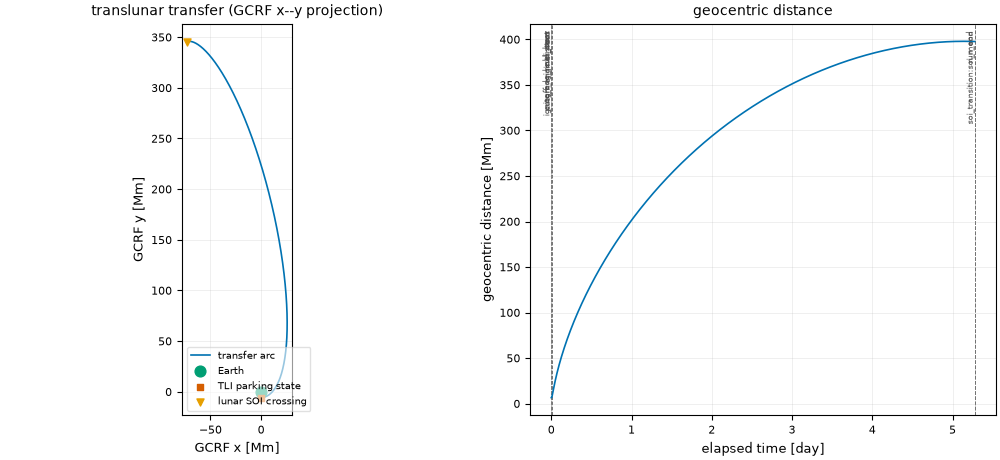
\includegraphics[width=\linewidth]{figures/translunar_transfer.png}
\caption{Translunar transfer from \texttt{missions/tli.toml}: GCRF $x$--$y$
  projection (left) and geocentric distance versus elapsed time with event
  markers (right). Regenerated bit-for-bit from the committed run by
  \texttt{scripts/figures/casestudy\_figures.py}; resolved-config
  SHA-256 prefix \texttt{4345078cfee2}.}
\label{fig:tli}
\end{figure}

\subsection{Earth--Mars transfer}
\label{sec:cases-mars}

The Earth--Mars case (\texttt{missions/mars\_cruise.toml}) propagates a
point-mass probe on a Hohmann-class heliocentric transfer about the Sun, under
the Earth, Moon, Venus, Mars, and Jupiter third bodies plus solar radiation
pressure, with the adaptive RKF7(8) integrator. Because the fixed-rate SRLOG
logs at a $\SI{1}{\hertz}$ floor, the committed mission propagates the first
seven days of the $\sim\!259$-day transfer after the escape handoff rather than
the full cruise, and the acceptance gate checks the osculating transfer ellipse
against Mars' orbital radii rather than arrival geometry. Figure~\ref{fig:mars}
shows the heliocentric arc and the osculating semi-major axis history: the
departure handoff sits at $\sim\!\SI{0.986}{\astrounit}$ from the Sun, and
Earth's residual pull draws the osculating semi-major axis down from
$\sim\!\SI{1.279}{\astrounit}$ toward the Hohmann aphelion target as the
spacecraft
recedes.

\begin{figure}[htbp]
\centering
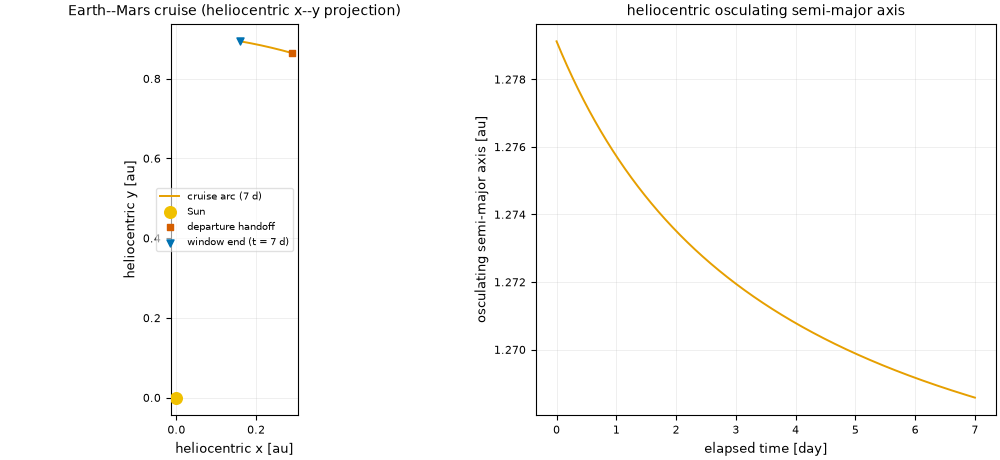
\includegraphics[width=\linewidth]{figures/mars_transfer.png}
\caption{Earth--Mars cruise from \texttt{missions/mars\_cruise.toml}:
  heliocentric $x$--$y$ projection over the committed seven-day window (left)
  and osculating semi-major axis versus elapsed time (right). Regenerated
  bit-for-bit from the committed run by
  \texttt{scripts/figures/casestudy\_figures.py}; resolved-config
  SHA-256 prefix \texttt{41819e7c4224}.}
\label{fig:mars}
\end{figure}

\subsection{Figure reproducibility}
\label{sec:cases-repro}

The case-study figures are a bit-for-bit regression artifact. With the pinned
matplotlib version and \texttt{SOURCE\_DATE\_EPOCH} set, the figure script
renders each PNG as a pure function of its committed decimated-run input and the
rendering toolchain: the Agg backend is forced before any display can be
touched, the matplotlib version string is dropped from the PNG metadata, and
the figure geometry and DPI are fixed in the script. Rendering each figure twice
in fresh processes produces byte-identical PNGs, verified by SHA-256; the
committed \texttt{translunar\_transfer.png} and \texttt{mars\_transfer.png}
carry SHA-256 prefixes \texttt{8be8e5052832} and \texttt{bc15057ddcf5}
respectively under the pinned matplotlib \texttt{3.11.1} and FreeType
\texttt{2.14.3}.
The pinned toolchain is recorded beside the script, because the rendered bytes
depend on both the plotting library and the font rasterizer; the runtime
dependency floor is \texttt{matplotlib>=3.8}, while the bit-for-bit guarantee is
against the exact pinned versions.

\section{Applications and Future Work}
\label{sec:applications}

The simulator is built as a research instrument for three uses: conventional
mission analysis; GNC algorithm development against a scrutinized truth model;
and world-model and machine-learning spacecraft-navigation research. The AI/ML
surface is present in the architecture from the outset, not bolted on: a
major-cycle stepping API suitable for reinforcement-learning loops with
zero-order-hold commands and adaptive-step termination on cycle boundaries;
seeded sensor emulation whose streams are bit-identical across reruns; a uniform
plugin interface that accepts Python and C++ GNC components interchangeably
through a single abstract base; consistency tooling that gates learned and
classical estimators alike on NEES and NIS statistics; and manifest-driven
batch generation whose NumPy export is the training-data interchange. A
Gymnasium adapter and an ONNX-runtime learned-controller path are the sanctioned
in-the-loop learned-model routes, and the interface truth boundary --- no route
carries evolving true state to a GNC component under a batch run --- is enforced
by construction and pinned by test.

Future work follows the phased roadmap to a completed validation campaign and to
the applications above. Two items are called out as explicitly pending. First,
cross-platform final-state divergence, bounded at $\le\!10^{-9}$ relative and
measured on
short reference arcs, must be re-measured on long heliocentric arcs where
transcendental-function differences accumulate, and the bound tightened or
per-regime-split as the data require. Second, the Raspberry~Pi~5 hardware
qualification --- the sub-\SI{60}{\second} cislunar and $\ge\!100\times$
real-time ascent performance gates, the offline viewer check, and the aarch64
cross-platform learned-model comparison --- is prepared as scripted,
committed procedures on the pre-release checklist but has not been executed on
Pi~5 silicon, because no such hardware is available to the maintainer at this
revision; a continuous-integration aarch64 leg gates these as a documented
proxy in the interim. Each of these is registered rather than silently waived.

\section{Conclusion}
\label{sec:conclusion}

\texttt{star\_reacher} pursues a deliberately narrow thesis: that a
six-degree-of-freedom space-mission simulator can be simultaneously small,
fully auditable, and reproducible to the bit, without sacrificing scientific
fidelity, and that such an instrument is the right substrate for
machine-learning navigation research because every training signal it emits
traces to a derived, cited, and tested model. The model set is complete through
the current phase and documented chapter by chapter; the acceptance suite passes
in full; seven cross-tool comparisons are measured inside their gates; and the
case-study figures regenerate bit-for-bit from committed seeds. The work that
remains --- the long-arc cross-platform divergence re-measurement and the
hardware qualification --- is specified, prepared, and registered rather than
assumed complete, in keeping with the project's honest-status discipline.

\printbibliography

\end{document}
